%%% Dateikodierung: UTF-8
%%% äöüÄÖÜß  <-- keine deutschen Umlaute hier? UTF-faehigen Editor verwenden!

%%% Magic Comments zum Setzen der korrekten Parameter in kompatiblen IDEs
% !TeX encoding = utf8
% !TeX program = pdflatex 
% !TeX spellcheck = de_DE
% !BIB program = biber

\documentclass[master,english,smartquotes]{hgbthesis}
% Zulässige Optionen in [..]: 
%    Typ der Arbeit: 'diploma', 'master' (default), 'bachelor', 'internship' 
%    Hauptsprache: 'german' (default), 'english'
%    Option zur Umwandlung in typografische Anführungszeichen: 'smartquotes'
%    APA Zitierstil: 'apa'
%%%-----------------------------------------------------------------------------

\RequirePackage[utf8]{inputenc} % bei Verw. von lualatex oder xelatex entfernen!

\graphicspath{{images/}}  % Verzeichnis mit Bildern und Grafiken
\logofile{logo}           % Logo-Datei: images/logo.pdf (kein Logo: \logofile{})
\bibliography{references} % Biblatex-Literaturdatei (references.bib)

%%%-----------------------------------------------------------------------------
% Angaben für die Titelei (Titelseite, Erklärung etc.)
%%%-----------------------------------------------------------------------------

%%%\title{Peer to Peer File Sharing Netzwerke}
%%%\author{Andreas Zauner}
%%%\programname{Software Engineering}

%\programtype{Fachhochschul-Bachelorstudiengang} % auswählen/editieren
%%%\programtype{Fachhochschul-Bachelorstudiengang}

%%%\placeofstudy{Hagenberg}
%%%\dateofsubmission{2021}{07}{15} % {YYYY}{MM}{DD}

%%%\advisor{Alois B.~Treuer, Päd.\ Phil.} % optional

%\strictlicense % restriktive Lizenz anstatt Creative Commons (nicht empfohlen!)

%%%-----------------------------------------------------------------------------
\begin{document}
%%%-----------------------------------------------------------------------------

%%%-----------------------------------------------------------------------------
\frontmatter                                       % Titelei (röm. Seitenzahlen)
%%%-----------------------------------------------------------------------------
 
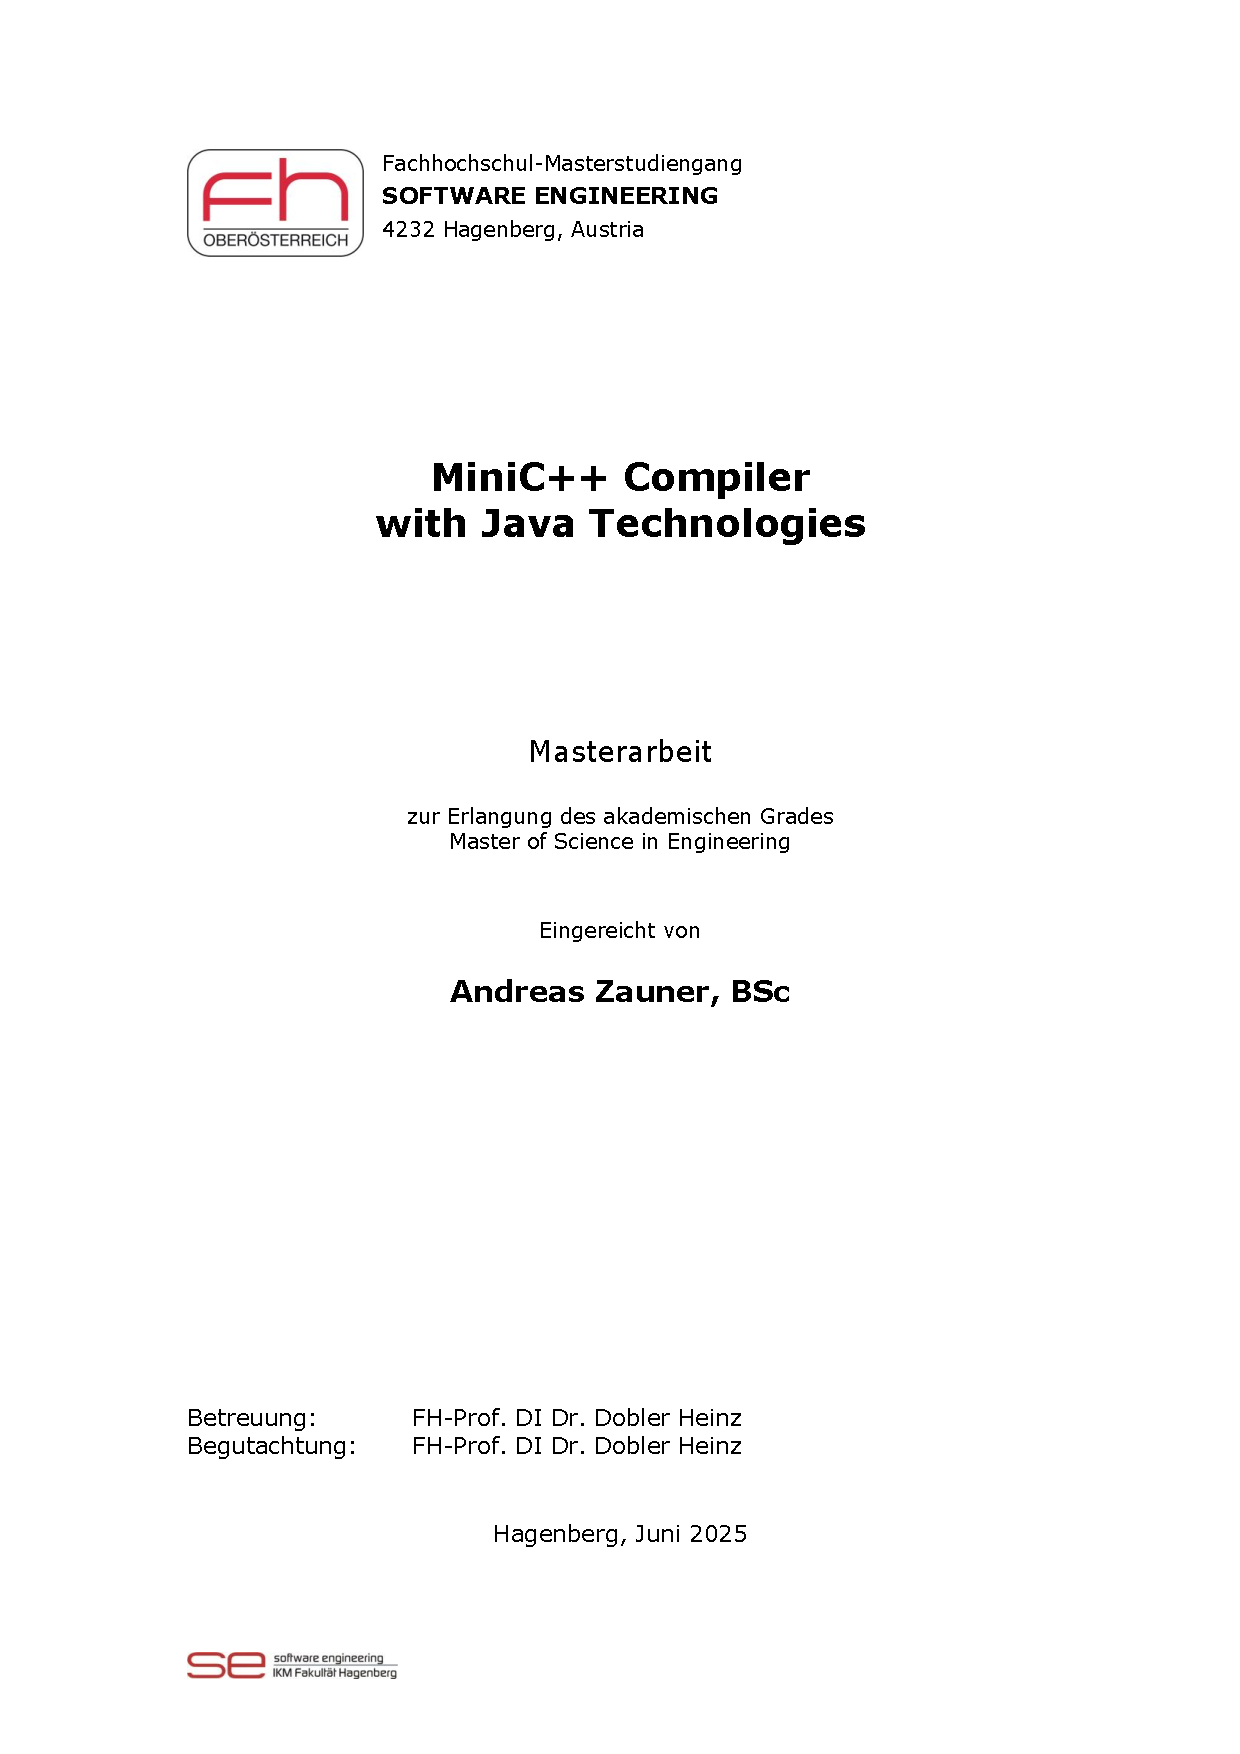
\includepdf[pages=1]{Titelblatt_Masterarbeit.pdf}
\includepdf[pages=2, pagecommand={\thispagestyle{plain}}]{Titelblatt_Masterarbeit.pdf}

\tableofcontents

\chapter{Kurzfassung}


\begin{german}

Diese Masterarbeit implementiert einen Compiler für MiniC\verb++| unter der Verwendung von Java-Technologien zur Erzeugung von Java-Bytecode. Für das Frontend wird der kombinierte Lexer- und Parsergenerator ANTLR verwendet, während das Backend die ObjectWeb ASM Bibliothek für die Bytecodegenerierung nutzt. Ähnlich zu Generatoren wie Coco-2 generiert ANTLR den Quellcode für einen Parser auf der Grundlage einer vorgegebenen Grammatik. ANTLR kann Code in mehreren Hostsprachen generieren; für diese Arbeit wurde Java gewählt. 

ANTLR ist ein Open-Source-Tool für die Spracherkennung. Es wurde erstmals 1992 veröffentlicht und wird seitdem von Terrence Parr kontinuierlich weiterentwickelt. In der aktuellen Version von ANTLR wird der adaptive-LL(*)oder ALL(*)-Parsing-Algorithmus verwendet. Dieser Algorithmus führt die Grammatikanalyse zur Parse-Zeit durch und überkommt dadurch die Einschränkungen früherer Versionen. ALL(*) erfordert nicht die Angabe einer maximalen Anzahl von Lookahead-Tokens. Stattdessen passt es sich an den aktuellen Kontext an und adaptiert die Anzahl der Lookahead-Token entsprechend.

Um einen abstrakten Syntaxbaum (AST) mit ANTLR zu erzeugen, werden drei Methoden unterstützt: Das Visitor-Pattern, das Listener-Pattern und die Verwendung einer attributierten Grammatik (ATG). Das Compiler-Frontend wird mit allen drei Methoden implementiert. Die drei Implementierungen werden in mehreren Aspekten verglichen und auf dieser Grundlage wird eine Empfehlung ausgesprochen.

ObjectWeb ASM ist eine in Java geschriebene Bibliothek zur Erzeugung von Java-Bytecode. Sie ist Open-Source und wird seit 2002 von Eric Bruneton entwickelt. Die Bibliothek wird in Compilern verwendet, die Java-Bytecode ausgeben, wie z.B. dem Kotlin-Compiler. Zur Generierung von Bytecode wird die auf dem Visitor-Pattern basierende API verwendet. 

Alle drei Frontend-Implementierungen sind mit dem Backend zu einer Anwendung verbunden, die Java-Bytecode aus MiniC\verb|++|-Code erzeugen kann. 

\end{german}
		
\chapter{Abstract}


\begin{english} %switch to English language rules
Peer-to-peer networks offer an alternative to the classic client-server model for exchanging data. In peer-to-peer networks, all clients communicate with each other. This means that the server, as the central element, can be omitted. This characteristic enables peer-to-peer networks to function even if individual participants in the network fail. In addition, peer-to-peer networks use the upload bandwidth of the individual clients, which is usually unused in traditional file sharing. 

This bachelor thesis deals in detail with peer-to-peer networks. First, known peer-to-peer networks are introduced and their characteristics are explained. Then it is shown where companies and organisations utilize peer-to-peer networks. A distinction is made between freely available networks and networks developed by companies themselves. Finally, a client for the BitTorrent network is developed. This client is able to exchange a file with other peers using the BitTorrent protocol. This shows how data exchange in a peer-to-peer network works on a technical level and which technologies are required for this.
\end{english}

			

%%%-----------------------------------------------------------------------------
\mainmatter                             % Hauptteil (ab hier arab. Seitenzahlen)
%%%-----------------------------------------------------------------------------

\chapter{Introduction}
\label{cha:introduction}

\section{Motivation}

Compilers are the backbone for computer programming. A compiler translates human-readable source code into something a computer can execute. This allows developers to focus on the functionality of the application, without having to worry about the technicalities of the concrete computer where the software will run on. For one programming language there may exist multiple compilers targeting different kinds of computers. This allows the same source code to run for example on Linux and Windows computers with Intel or ARM processors. This flexibility saves developers a lot of work, because they don't need to rewrite their application in the case they also want to target another operating system and/or processor. Furthermore, there exist compilers that target virtual machines like the Java Virtual Machine (JVM)\footnote{https://openjdk.org/groups/compiler/}. Generating code for a virtual machine has the advantage that there is no need for compilers for every target operating system and/or processor. Instead, for each operating system an implementation of the virtual machine is provided.

The process of compiling source code begins in the frontend of the compiler. The frontend reads the source code and constructs an abstract syntax tree (AST). The AST is a representation of the source code in memory. It contains only the necessary information that is needed to generate target code. The process of constructing the AST is based on the grammar of the programming language. Based on this grammar a lexer and parser are either written manually or get generated by a parser generator tool like ANTLR. In the case of ANTLR the generated lexer and parser by default construct a full parse tree from the input. From the parse tree an AST can be constructed using for example the visitor pattern. 

The AST functions then as the input for the backend of the compiler: The backend generates code for the target system. In the case of the JVM this is the so called bytecode.  APIs exist that provide an abstraction layer for the code generation. One API for bytecode generation is the open source project ObjectWeb ASM or just ASM \parencite{bruneton2007asm}. It provides an API that utilizes the visitor pattern to generate bytecode instructions. 


\section{Task and Goal}

MiniC++ is a subset of the C++ programming language. The scope of MiniC++ is very limited in comparison to C++. It is used at the University of Applied Sciences Upper Austria in Hagenberg for teaching software engineering master students about compilers in the formal languages class. In this class, all aspects of a compiler are discussed. First, the principles of lexers and parsers are explained. Then the concepts of syntax trees and further abstract syntax trees are introduced. Finally, code generation is explained. 

In the exercises, students use a MiniC++ compiler to compile MiniC++ source code to the .NET Common Intermediate Language (CIL). The frontend of the compiler is generated by using the compiler generator Coco-2 \parencite{doblerCoco2}. Which generates both, the lexer and the parser. There is only one input-file required for the definition of the lexer and the parser. Furthermore, attributes and semantic actions can be included to create an attributed grammar (ATG). 

In this master thesis, another compiler for MiniC++ will be created. This compiler will be built upon Java technologies. Output of the compiler will be Java bytecode that can be executed on the Java Virtual Machine (JVM). The frontend is based on a lexer and parser generated by the parser generator ANTLR\footnote{https://www.antlr.org/} (ANother Tool for Language Recognition). They are used to generate a full syntax tree. From this syntax tree an abstract syntax tree (AST) is constructed. The backend utilizes the ObjectWeb ASM\footnote{https://asm.ow2.io/} library. This library provides an API to generate Java bytecode. 

This master thesis will further explore the capabilities of ANTLR. ANTLR provides multiple ways to interact with the generated parser. The master thesis compares the advantages and disadvantages of each of these options.

\section{Theoretical Fundamentals}

This section explains the basic concepts of formal languages and how they are used in compilers. Furthermore, the individual components of a compiler are highlighted. 

\subsection{Formal Languages and Compilers}

Formal languages make up the fundament on which compilers are built upon. In comparison to natural languages, formal languages have a strict syntax which can be defined by a grammar. This grammar does not evolve naturally, as it does with natural languages. A formal grammar is defined by replacement rules. A replacement rule defines that a non-terminal symbol \textit{A} can be replaced by a sequence $\alpha$. The sequence may contain terminal and/or non-terminal symbols. 

Grammars can be classified according to the Chomsky hierarchy \parencite{CHOMSKY1959137}. Chomsky classifies formal languages and their grammars into four categories. Of those, the first two are relevant for compiler construction. Namely, regular grammars and context-free grammars. The four categories are differentiated by the type of rules that can be defined. The types of rules used then define which kind of automaton is needed to recognize sentences of the given language. 

\subsubsection{Regular Grammars}

Regular grammars make up the simplest group of grammars. For a grammar to be regular all rules must be in the form of $A\rightarrow a | a B$ or $S\rightarrow \epsilon$. This means that a non-terminal symbol $A$ can only be replaced by either a terminal symbol $a$ or a terminal symbol $a$ followed by a non-terminal symbol $B$. The only exception is the root rule $S$ which can be replaced by the empty sequence. 

To recognize a sentence of a regular grammar a finite automaton (FA) can be used. A deterministic FA (DFA) consists of the following elements:

\begin{itemize}
    \item $S$ finite, non-empty set of states,
    \item $\Sigma$ finite, non-empty set of symbols (alphabet),
    \item $s_0$ initial state, $s_0 \in S$,
    \item $\delta$ state transition function, $S \times \Sigma \rightarrow S$ and
    \item $F$ set of final states, $F \subseteq S$.
\end{itemize}

The DFA proceeds to read the symbols in $\Sigma$ one symbol at a time. The current symbol is then used in combination with the current state in the state transition function to acquire a new state. This process is continued until a final state is reached, meaning that a sentence has successfully been recognized. In case that for the current symbol and state no entry in the state transition function can be found, the recognition failed, and the given input is not a sentence of the language. 

A DFA can be implemented in a program to efficiently recognize sentences of a language. For more complicated regular languages nondeterministic finite automata (NFA) are easier to construct. A NFA program however is more complicated and slower compared to a DFA one. Every NFA can be transformed to a DFA to overcome this limitation. After transformation the constructed DFA may have more than the minimal number of states needed. A second transformation can be performed that reduces the DFA to a minimal DFA. 

\subsubsection{Context-Free Grammars}

Context-free grammars are the second group of grammars according to the Chomsky hierarchy. Context-free grammars include regular grammars, meaning that every regular grammar is also a context-free grammar. A replacement rule of a context-free grammar is in the form $A \rightarrow \beta$. Meaning that a non-terminal symbol $A$ can be replaced by a sequence $\beta$ containing terminal and/or non-terminal symbols or also $\varepsilon$, the empty sequence. 

In a context-free grammar central recursion is possible (direct or indirect). This allows the nested structures that are needed for programming languages, e.g., for expression hierarchies. Central recursion cannot be handled by a FA, for this a pushdown automaton (PDA) is needed. With a deterministic pushdown automaton (DPDA) all deterministic context-free grammars can be recognized. To recognize all context-free grammars a nondeterministic pushdown automaton (NPDA) is needed. For programming languages deterministic context-free grammars are used. 

There are two strategies for constructing a syntax tree from a sentence of a context-free grammar, namely top-down and bottom-up. Which strategy can be used depends on the kind of deterministic context-free grammar that is used. Following are the two most important conditions for context-free grammars:

\begin{itemize}
    \item \textbf{LL($k$) Condition:} Defines that a maximum of $k$ symbols look ahead are sufficient to deterministically decide on the next rule when using the \textit{top-down} strategy.
    \item \textbf{LR($k$) Condition:} Defines that a maximum of $k$ symbols look ahead are sufficient to deterministically decide on the next action(shift or reduce) when using the \textit{bottom-up} strategy.
\end{itemize}

The higher the value of $k$, the more complicated parsing becomes. Therefore, LL($1$) and LR($1$) grammars are preferred. For an LL($1$) or LR($1$) grammar only one symbol look ahead is needed for a deterministic decision. 

LL($k$) grammars can be recognized with a normal DPDA. For LL($1$) grammars it is also feasible to implement an efficient recursive descent parser. In the case of an LR($1$) grammar, the DPDA must be extended to be able to use an arbitrary amount of symbols on top of the stack. Only then is it able to recognize a sentence of an LR($1$) grammar with the \textit{bottom-up} strategy. It has to be noted that a DPDA which is able to recognize LR($k$) grammars, is also able to recognize LL($k$) grammars.

\subsection{Compiler Construction}

The task of a compiler is to translate code of a given source language into code of a target language. The source language being a human-readable programming language like Java and the target language being code for a given operating system and processor architecture, or a virtual machine. Compiling code can be separated into two main stages: frontend and backend.
The frontend executes of the following steps:
\begin{itemize}
    \item lexical analysis,
    \item syntactic analysis,
    \item semantic evaluation and
    \item intermediate language generation.
\end{itemize}

The backend performs optimization and code generation.

%\subsubsection{Lexical Analysis}
The lexical analysis is the first step of the compilation. It reads the source code and organizes it. The goal is to group individual characters into symbols and to skip meaningless characters (e.g., comments). The grammar of the source language provides the information about the symbols. This part of the grammar is defined using a regular grammar. 

The symbols can be divided into terminal symbols and terminal classes. Terminal symbols are special symbols like \texttt{=}, \texttt{(}, \texttt{-} and the keywords of the source language, e.g., \texttt{int}, \texttt{break},  \texttt{function}. Terminal classes are for example all numbers or identifiers. Comments are also handled at this step. Since comments usually have no influence on the generated code, they are removed. All recognized symbols are then passed to the parser (syntactic analysis and semantic evaluation). 


%\subsubsection{Syntactic Analysis}

The syntactic analysis takes the terminal symbols and classes recognized in the lexical analysis phase as input to construct the syntax tree. A context-free grammar provides the basis for the syntax tree. During the syntactic analysis the terminal symbols are grouped into syntactic elements according to the grammar. Furthermore, the syntactic integrity is also checked. In case that there is no grammar rule available for the current terminal symbol, the syntactic analysis fails, and a syntax error is reported.

%\subsubsection{Semantic Evaluation}

According to the principle of syntax-directed parsing, during the syntactic analysis the semantic evaluation is performed. This may include constructing the abstract syntax tree (AST). In the AST only the relevant information for the code generation is contained. For each rule in the grammar, there may be semantic actions associated with it, that get executed when the rule is visited. The semantic actions have access to the attributes of the rule. This information is used to generate the AST.  

%Taking the AST as a basis, the intermediate language code generation is performed. This includes for example generating the symbol table. 

Afterwards, the intermediate language code is analyzed and optimized. This may include optimizations such as inlining or loop unrolling. Depending on the use case, more aggressive optimizations can also be performed. 

Finally, the code generation unit takes the optimized code and generates the appropriate instructions for the target language. 
\chapter{Methods and Tools for Compiler Frontends}

In this chapter  methods and tools for the construction of compiler frontends are explained. This explanation is focused on the parser generator ANTLR. The basis for this chapter is the book "The Definitive ANTLR 4 Reference" by \textcite{Antlr4Reference}.

\section{Attributed Grammars}

Parser generators like ANTLR or Coco-2 require the definition of the grammar of the source language in a specific format. These formats also allow for the declaration of attributes and semantic actions in the grammar. Semantic actions have access to the attributes of symbols (terminal and non-terminal) of a rule. Some symbols have attributes associated with them. The combination of a grammar, attributes and semantic actions is called an attributed grammar.  


There are two types of attributes: inherited and synthesized attributes. The former ones are computed based on the attributes of the parent node. Synthesized attributes are based on the attributes of the children nodes.  
The type of attributes available depends on the parsing strategy. For a top-down strategy the attributes of child-nodes are not available, as they have not been parsed yet. Conversely, when using the bottom-up strategy, the attributes of parent nodes are not available. 

Especially relevant are the attributes of terminal classes. Through the attribute of a terminal class like \texttt{number}, the actual number that this class node holds can be accessed. These kinds of attributes are provided by the lexical analyzer. 

In listing \ref{lst:Coco2ATG} a simple attributed grammar for Coco-2 for arithmetic expressions is shown. This grammar uses semantic actions to calculate the result of an arithmetic expression. Semantic actions are encoded inside \lstinline{SEM<< >>} blocks; in this case C\verb|#| code. Synthesized attributes provide the results of the calculations from the child nodes. These attributes are available inside the semantic actions where the actual calculation is performed. 

While it is convenient to embed semantic actions directly into the grammar, it is not without disadvantages. By embedding code of a specific language, it is no longer possible to use the same grammar to generate a parser in another implementation language. Parser generators like ANTLR provide multiple implementation languages to generate a parser for. 

\begin{GenericCode}[float,numbers=none,caption=Attributed Grammar for Coco-2 for simple arithmetic expressions., label=lst:Coco2ATG]
Expr<<out int e>> =    LOCAL<<int t = 0; e = 0;>>
  Term<<out e>>             
  { '+' Term<<out t>>    SEM<<e = e + t;>>
  | '-' Term<<out t>>    SEM<<e = e - t;>>
  }.

Term<<out int t>> =    LOCAL<<int f = 0; t = 0;>>
  Fact<<out t>>
  { '*' Fact<<out f>>  SEM<<t = t * f;>>
  | '/' Fact<<out f>>  SEM<<t = t / f;>>
  }.
  
Fact<<out int f>> =    LOCAL <<f = 0;>>
    number<<out f>>
  | '(' Expr<<out f>> ')'.

\end{GenericCode}

\section{ANTLR}

In this section, the parser generator ANTLR (ANother Tool for Language Recognition) is explained. First, a general overview of the history of ANTLR is given, followed by the introduction of the parsing algorithm currently employed by ANTLR, namely ALL(*). Finally, the general functionality of ANTLR is explained.  

\subsection{History}

"ANTLR (ANother Tool for Language Recognition) is a powerful parser generator for reading, processing, executing, or translating structured text or binary files". As the acronym of ANTLR states, it is a tool for language recognition. ANTLR was first released in 1992 and has since then been in continuous development. The original creator and maintainer of the project is Terence Parr. ANTLR is written in Java and is open sourced under the BSD license. Its source code can be viewed on GitHub\footnote{https://github.com/antlr/antlr4}. 

Many projects utilize ANTLR. Notable examples include the Java Object-Relational Mapping tool \cite{HibernateWeb2024} and the NoSQL database Apache \textcite{Cassandra2024}.

ANTLR originally started of as the master thesis of Terrence Parr \parencite{PCCTSHistory1994}. A first alpha release was created in 1990, that only generated LL(1) parsers. Version 1 of ANTLR incorporated the new parsing algorithm developed by Parr that allowed to create parsers for LL(k) grammars \parencite{parrPhd1993}. Version 2 then provided incremental improvements.   

Version 3, released in 2006 introduced a new parsing algorithm called LL(*) \parencite{LLSParsing2011}. The LL(*) parsing strategy performs parsing decisions at parse-time with a dynamic lookahead. The number of lookahead tokens increases to an arbitrary amount and decreases again using backtracking. However, the maximum amount of $k$ lookahead tokens still needs to be specified. Version 3 also introduced ANTLRWorks\footnote{https://www.antlr3.org/works}, a graphical IDE for the construction of ANTLR grammars.

The current version 4, released in 2013 again introduced a new parsing algorithm adaptive-LL(*) or ALL(*). The most significant improvement of ALL(*) over LL(*) is that the maximum number of lookahead tokens no longer needs to be specified. ANTLR v4 added support for the visitor and listener patterns\footnote{https://github.com/antlr/antlr4/blob/dev/doc/listeners.md}, enabling easier interaction with the syntax tree. 

\subsection{Parsing Algorithm Adaptive-LL(*)}
\label{sec:allstar}

The Adaptive-LL(*) or ALL(*) parsing strategy is introduced in the paper "Adaptive LL(*) parsing: the power of dynamic analysis" by \textcite{ALLParsing2014} and is the basis for this section. This parsing algorithm is used  for ANTLR version 4. As the title suggests, ALL(*) performs the analysis of the grammar at parse time. 

\subsubsection{Limitations of LL(*) Parsing Algorithm}

To understand the need for ALL(*), it is necessary to highlight why the previous strategy LL(*) is insufficient. LL(*), introduced by \textcite{parr2011ll}, was developed as an improvement to the existing general LL (GLL) \parencite{GLL2010} and general LR (GLR) \parencite{tomita1991generalized} parsers. For ambiguous grammars these parsers return multiple parse trees, which are undesirable for parsers of programming languages. GLL and GLR are  designed for natural languages, which are inherently ambiguous. LL(*) overcomes these limitations by using regular expressions that are stored inside a deterministic finite automaton (DFA) to offer mostly deterministic parsing. Using the DFA allows for regular lookahead even though the grammar itself is context-free. 

However, the LL(*) grammar condition cannot be checked statically, leading to the case that sometimes no regular expression is found that distinguishes the possible productions. Such situations are detected by the static analysis and then backtracking is used instead. Backtracking however comes with the disadvantage that for rules in the format $A \rightarrow a | ab$, the second alternative will never be matched, since backtracking always chooses the first alternative. 

\subsubsection{Dynamic Grammar Analysis with ALL(*)}

With ANTLR version 4 the parsing strategy Adaptive-LL(*) or ALL(*) was introduced. The main difference to ANTLR version 3 is that the grammar analysis is now performed at parse-time, and is no longer static. This overcomes the limitations of the static analysis LL(*) performs and enables the generation of correct parsers for context-free grammars. The only exception are grammars that contain indirect or hidden left-recursion\footnote{Indirect left-recursion is a rule like $A \rightarrow Bx, B \rightarrow Ay$. $\epsilon$ productions cause hidden left-recursion. Take a rule $B \rightarrow \epsilon$ that produces only the empty chain $\epsilon$ and another rule $A \rightarrow BA$. Since B's only production is to $\epsilon$ the second rule causes a left-recursion. }. From an engineering perspective it was seen to be too much effort, since these grammars are deemed to be not common. Direct left-recursion is possible, because ANTLR rewrites the grammar to be non-direct left-recursive before passing it to the ALL(*) parsing algorithm. 

At a decision point (a rule containing multiple alternatives), ALL(*) starts a subparser for each alternative in pseudo-parallel. A subparser tries to match the remaining input to the selected alternative. If the input does not match, the subparser dies off. All subparsers process one symbol at the time in pseudo-parallel. This guarantees that the correct alternative can be found with minimum lookahead. In the case of ambiguity due to multiple subparsers reaching the end of file or coalescing, the first alternative will be chosen. 

The performance of ALL(*) is improved by employing a cache. This cache is implemented in the form of a DFA. The DFA stores the same information as the DFA generated by LL(*) from static analysis. After a lookahead, the DFA stores which production resulted from the lookahead phrase. If at a later time the same lookahead phrase is being processed, the correct production can be retrieved from the DFA. Theoretically, a DFA is not able to recognize a context-free grammar, however due to the analysis being performed at parse time, the analysis only needs to be performed on the remaining input. Since the remaining input is a subset of the context making it regular. Another optimization is the usage of a graph-structured stack (GSS). The GSS makes sure that during the prediction, no computation is performed twice, effectively acting as a cache. 

%In some cases it is necessary for ALL(*) to examine the parse stack to make a decision. 
%section about SLL
The theoretical runtime complexity of ALL(*) is $O(n^4)$. This stems from the fact that in the worst case the ALL(*) parser needs to make a prediction for each symbol and each launched subparser then needs to inspect the entire remaining input. In practice ALL(*) performs linearly for common programming languages like Java or C\verb|#|.


\subsection{Functionality}

ANTLR generates a combined lexer and parser from a single grammar file. The generated parser is a recursive descent parser. ANTLR supports various implementation languages such as Java, C\verb|#| or C++. The syntax used by the ANTLR grammar supports extended BNF (EBNF) operators such as \texttt{?}. To interact with the generated parser, ANTLR optionally generates interfaces and implementations for the listener and visitor pattern.

ALL(*) does not use a separate lexical analysis phase. Instead lexical and syntactical analysis are integrated into a unified process. Lexical rules are treated as parser rules, therefore a separate lexical analysis phase is not needed. Since the phases are combined, it is possible for ALL(*) to perform context-sensitive lexing. The lexer can make a decision based on the current parsing context. The parsing is directly performed on the raw input stream and not on a separate token stream. 

\subsubsection{Semantic Predicates}

ANTLR supports the definition of so-called \textit{semantic predicates}. Semantic predicates are boolean expressions, defined in the host language that allow for the dynamic alteration of the language generated by the grammar. If a semantic predicate is present for a production, the production can only be accepted if the semantic predicate evaluates to true. Semantic predicates are expressed inside \verb|{ }| parenthesis followed by $?$. Listing \ref{lst:ANTLRSemPred} illustrates an example use case of a semantic predicate. The rule \texttt{blockEnd} contains a semantic predicate specifying that the production can only be accepted if there is currently a block on the stack. 

A semantic predicate also has access to the current token. This enables conditions that directly interact with the input. For example separate productions for even and uneven numbers could be used. The semantic predicate then checks if the number is even or not.  


\subsubsection{Semantic Actions}

In ANTLR grammars semantic actions can be defined. Semantic actions can be inserted in every parser rule, before, in between and after symbols. Similar to semantic predicates, the semantic action is to be defined in the implementation language. Semantic actions are defined inside \verb|{ }| parenthesis. To access a symbol the name of the symbol prefixed by \verb|$| can be used. In Listing \ref{lst:ANTLRSemPred} semantic actions are used in the \texttt{blockStart} \texttt{blockEnd} rules. For the \texttt{blockEnd} it has to be noted that semantic predicates and actions can be used together. 

% semantic actions

\begin{AntlrCode}[float,numbers=none,caption=Example grammar using a semantic predicate and a semantic action., label=lst:ANTLRSemPred]
grammar Example;
@members {
    java.util.Stack<String> blockStack = new java.util.Stack<>();
}

program: statement* EOF;

statement
    : blockStart
    | blockEnd
    | otherStatement
    ;

blockStart: 'begin' { blockStack.push("block"); };

blockEnd: 'end' { !blockStack.isEmpty() }? { blockStack.pop(); };

otherStatement: 'print' IDENTIFIER;

IDENTIFIER: [a-zA-Z_][a-zA-Z_0-9]*;

WS  : [ \t\r\n]+ -> skip;
\end{AntlrCode}


\subsubsection{Alternative Labels for Rule Alternatives}

Per default ANTLR generates one method for each rule. In the case of multiple alternatives for a rule, the handling of the alternatives would need to be done manually. Therefore, ANTLR offers the possibility to attach a label to each of the alternatives. Then a method for each alternative will be generated separately. One use case is highlighted in listing \ref{lst:ANTLRRuleAlt}. The rule \texttt{type} matches to either one of the four types. Each alternative has a label associated to it by using \verb|#| as the prefix for the alternative name. With this definition four methods will be generated corresponding to each of the alternatives as explained above.     

\begin{AntlrCode}[float,numbers=none,caption=Example rule using alternative labels for the rule alternatives., label=lst:ANTLRRuleAlt]
  type
      : 'int'     #IntType
      | 'bool'    #BoolType
      | 'long'    #LongType
      | 'string'  #StringType
      ;
\end{AntlrCode}

\section{Syntax Tree and Abstract Syntax Tree (AST)}

A syntax tree is a hierarchical representation of the syntactical structure of a sentence. Also referred to as a parse tree, this representation is usually generated by a parser. A syntax tree contains the information of the entire sentence based on the grammar of that language. Each inner node in the syntax tree corresponds to a rule in the grammar. The leaf nodes represent terminal symbols and inner nodes are non-terminal symbols. Concatenating the leaf nodes from left to right of the syntax tree results in the original sentence from which the syntax tree was constructed from. 

Listing \ref{lst:SyntaxTreeEx} shows the syntax tree of the arithmetic expression \texttt{5 * 3 + 7} based on the grammar in \ref{lst:Coco2ATG}. 
%TODO
This syntax tree contains the non-terminal symbol \texttt{Expression, Term, Fact} and the terminal class \texttt{number}. The expression is built from two terms and one operator. The left term represents a multiplication consisting of two factors and an operator. All factors in the syntax tree contain the terminal class \texttt{number} which hold the concrete numbers. This structure further enables the representation of the precedence rules of arithmetic operations directly in the syntax tree.  

\subsection{Abstract Syntax Tree (AST)}
In an abstract syntax tree (AST) only a subset of the nodes from the original syntax tree are included. The goal is to focus on the semantic aspects of the syntax tree. Syntactical details, e.g., semicolons are omitted. 

The generation of an AST from a syntax tree can be done in multiple ways. One method is to generate the AST during the parse, which increases performance since the syntax tree does not need to be traversed twice. This can be implemented by using an attributed grammar with semantic actions that embed the AST generation code directly into the parser. Parsers like ANTLR also support the listener pattern to execute code during the parse. Alternatively the AST can be generated after the parse phase from the syntax tree. To traverse the syntax tree the visitor pattern can be used for example.  

The AST is then used in the subsequent stages of a compiler. This transformation is performed to create a new tree which omits all information that is of no importance to the following stages of the compiler. Subsequent code optimization may further slim down the AST. 

Continuing with the previous example, listing \ref{lst:ASTEx} shows the AST of the arithmetic expression \texttt{5 * 3 + 7}. This AST still contains the same semantic meaning as the full syntax tree, however it needs fewer nodes for that. Instead of using the non-terminal symbols, the operator is used, effectively encoding the same information. In this example, the node count can be reduced from 14 to 5.

\begin{GenericCode}[float,numbers=none,caption=Syntax tree of the arithmetic expression \texttt{5 * 3 + 7} based on the grammar in listing \ref{lst:Coco2ATG}., label=lst:SyntaxTreeEx]
                                       Expr   
                                   /    |    \
                                Term    +    Term
                              /   |   \        |    
                           Fact   *   Fact    Fact  
                            |          |       |
                          number     number  number
                            |          |       |
                            5          3       7
\end{GenericCode}

\begin{GenericCode}[float,numbers=none,caption=Abstract syntax tree of the arithmetic expression \texttt{5 * 3 + 7}., label=lst:ASTEx]
                                      +
                                    /   \
                                   *     7
                                 /   \
                                3     5
\end{GenericCode}

\section{Visitor-Pattern for Tree Transformation}

In the case that a syntax tree is already present, the visitor-pattern can be used to create an AST from the syntax tree. Using the visitor-pattern, the syntax tree gets traversed and then step by step the AST is constructed. The visitor-pattern allows for the separation of algorithms from the objects they operate on. Instead of including the code for the generation of an AST object in the syntax tree object, a separate object, a so-called \textit{visitor} is taking care of this. 

To implement visitor-pattern for a syntax tree, the best approach is to use interfaces or abstract classes for the nodes of the syntax tree and the visitors. Listing \ref{lst:ListPatIntEx} shows a possible implementation for an interface and abstract class in Kotlin. This code is based on the syntax tree shown in listing \ref{lst:SyntaxTreeEx}. Each class of the syntax tree implements the  abstract class \texttt{SyntaxTreeNode}. For the visitor class the \texttt{SyntaxTreeVisitor} interface needs to be implemented. Both classes are generic. This allows the implementation of the visitor to use an arbitrary type as a return value. Multiple visitors can then be implemented using the generics, so that each visitor can return one type of the AST types. In this case it is helpful to create an abstract base visitor that provides an empty implementation for all interface's methods. Then the concrete visitor only needs to override the methods that are relevant for the specific AST type.  

A \texttt{SyntaxTreeNode} can then be visited by calling its \texttt{accept} method. Inside the \texttt{accept} method, the appropriate method of the \texttt{SyntaxTreeVisitor} will be called. As can be seen in listing \ref{lst:ListPatNumbNode} the \texttt{NumberNode} calls the \texttt{visitNumberNode} with itself as the parameter. This behavior is analogous for all other nodes of the syntax tree. 


\begin{KotlinCode}[float,numbers=none,caption=Interface and abstract class used to implement the visitor-pattern., label=lst:ListPatIntEx]
sealed class SyntaxTreeNode {
    abstract fun <T> accept(visitor: SyntaxTreeVisitor<T>): T
}

interface SyntaxTreeVisitor<T> {
    fun visitNumberNode(node: NumberNode): T
    fun visitOperatorNode(node: OperatorNode): T
}
\end{KotlinCode}


\begin{KotlinCode}[float,numbers=none,caption=Implementation of the \texttt{NumberNode} class inheriting from the \texttt{SyntaxTreeNode}., label=lst:ListPatNumbNode]
  data class NumberNode(val value: Int) : SyntaxTreeNode() {
    override fun <T> accept(visitor: SyntaxTreeVisitor<T>): <T> {
        return visitor.visitNumberNode(this)
    }
}
  \end{KotlinCode}


\section{Listener-Pattern for Tree Transformation}

The listener-pattern is used for \textit{listening} to events or notifications from another object. In the context of parsing, the listener-pattern is used to handle parse events coming from the parser. This includes events such as entering and exiting a node during the parse. When using the listener-pattern the parse tree is only traversed once. This is because the events get pushed to the listeners during the parse. 

To implement the listener-pattern for the construction of an AST, a listener interface is needed. The listener interface contains method declarations for entering and exiting each node type. The methods take the syntax tree node as the input parameter. A possible implementation for the listener interface is shown in.  In case of the \textit{enter} methods, the symbols for the syntax tree node have not been parsed yet, so no data from them is available yet.

A concrete listener will then implement the interface and register/subscribe itself to the events of the parser. When the parser enters or exits a node during parse it will call the respective method with the parsed syntax tree node for all listeners. 

\begin{KotlinCode}[float,numbers=none,caption=Implementation of the \texttt{ExpressionListener} interface., label=lst:ListPatExprList]
interface ExpressionListener {
    fun enterExpr(node: Expression)
    fun exitExpr(node: Expression)

    fun enterNumer(number: Number)
    fun exitNumber(number: Number)
}
  \end{KotlinCode}





%%%-----------------------------------------------------------------------------
\appendix                                                               % 

%%%-----------------------------------------------------------------------------
\backmatter                          % Schlussteil (Quellenverzeichnis und dgl.)
%%%-----------------------------------------------------------------------------

\MakeBibliography % Quellenverzeichnis
%%%-----------------------------------------------------------------------------
\end{document}
%%%-----------------------------------------------------------------------------
